\section{Results}

Based on the findings of~\cite{withInsects}, several performance and configuration aspects of the 
proposed sensor can be deduced. Those relate to both the feasibility of the proposed sensor in order
to extract relevant information from the scene, as well as application areas for different configurations
of the honeycomb pattern.

\begin{figure}[t]
    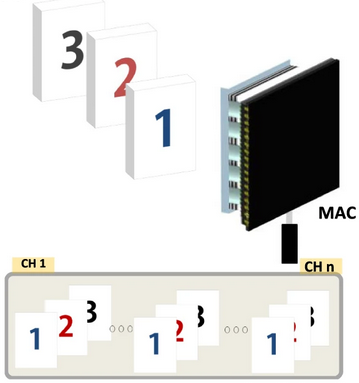
\includegraphics[width=0.50\textwidth, height=0.50\textwidth]{resources/png/paper_result.png}
    \caption{Visual disparity showcase.~\cite{withInsects}~\label{figResults}}
\end{figure}

Firstly, as shown in~\ref{figResults}, there is enough distinction
between the images captured by each sensing areas, such that disparity-based can be utilized in order
to extract 3-dimensional information. While the example only showcases horizontally spaced sensors, 
the hexagon-based proposal will have three main axes in which the scene will be assessed, further
increasing the accuracy of the system.

\begin{figure*}[t]
    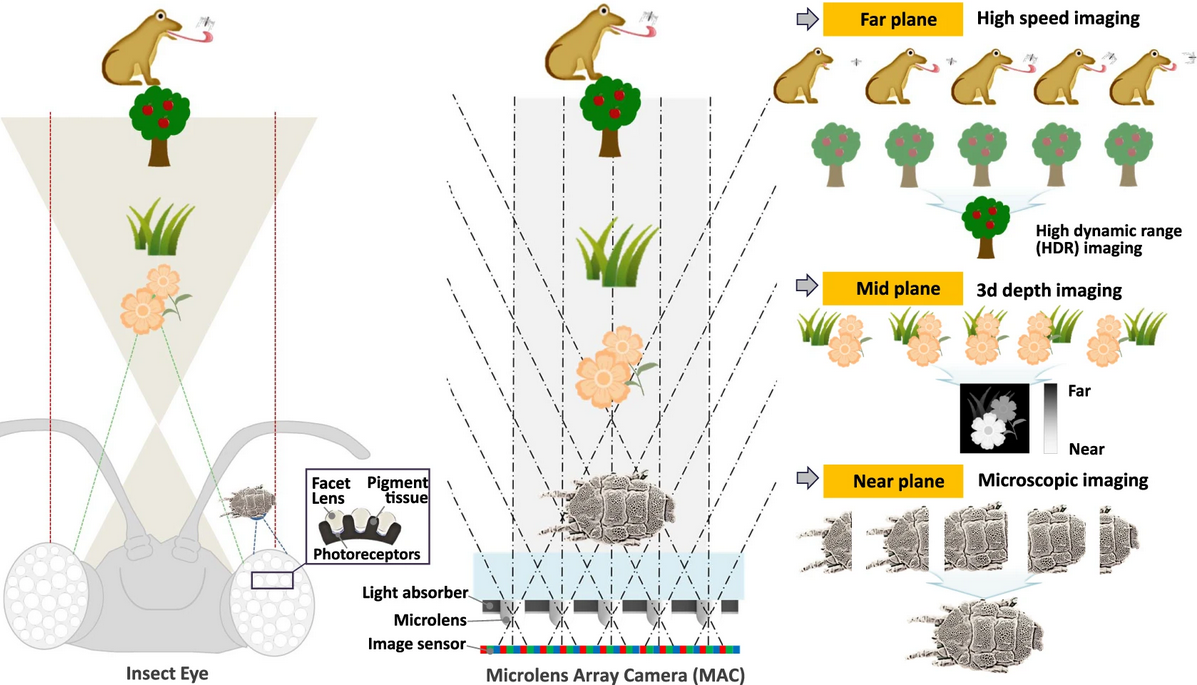
\includegraphics[width=1.0\textwidth, height=0.50\textwidth]{resources/png/paper_working.png}
    \caption{Multiple stereopsis example.~\cite{withInsects}~\label{figWorking}}
\end{figure*}

Secondly,~\ref{figWorking} presents the different use cases for multiple stereopsis systems. Due to
the configurability of the proposed system, it could be adapted to function in different environments,
with the most relevant environment being close-range imaging, due to the distance between image planes
being equal to the size of the images themselves. As this is entirely dependent on the desired resolution
and particular sensor configuration, use cases might range from surgery assistance to vehicle automation.